\graphicspath{{./figures}}

\section{High-Level System}
There are various decisions to be made regarding the entire communication system. A complete high-level system block diagram illustrating the decisions discussed below is shown in Figure \ref{fig:complete_system}. Note that the yellow blocks are external (i.e. assumed to be available already).

\begin{figure}[!htb]
    \centering
    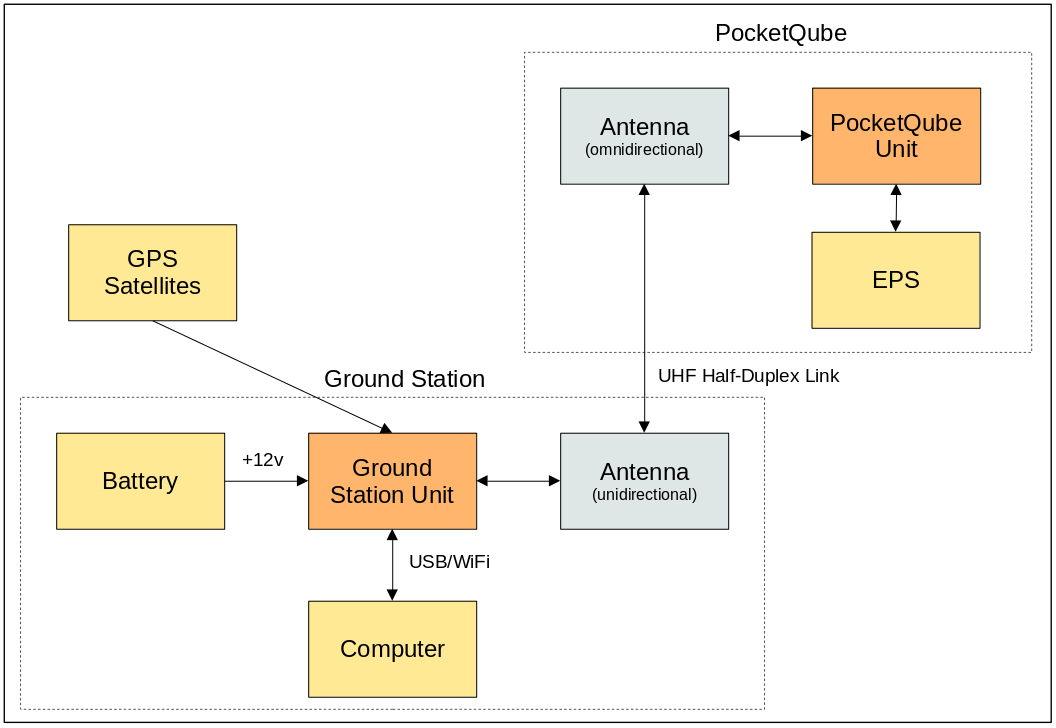
\includegraphics[width=0.8\textwidth]{complete_system.png}
    \caption{High-Level System Diagram}
    \label{fig:complete_system}
  \end{figure}

\newpage
\subsection{Methodology}
Since a large number of sub-systemS are required on the ground-station, either IC \textit{modules} or simple \textit{reference designs} will be form the basic building blocks of the system. This will simplify the design process and integration. Only if no modules or designs are found to meet the system requirements, should a more custom solution be developed. The ground station will be powered via +12V from a nearby vehicle, and the PocketQube will be powered from an on-board EPS (another PQ unit). Both sub-systems should be designed such that testing without a vehicle/EPS is also possible.

\subsection{Tracking}
It is assumed that open-loop path-predicted tracking is generally adequate for high-altitude balloons, given the number of tools available to predict their flight path. In this sense, the ground station requires at least a GPS connection, as well as a means of determining true north (such as a magnetometer) for beem steering. The path data will be uploaded to the ground station via USB from a system \textit{computer}. Further, this computer will be used to monitor the link and record the data. If time allows, direct GPS tracking will be added as a method of "closing the loop", and to improve pointing accuracy.

\subsection{Custom Protocol}
Half-duplex communication will be designed for, since full-duplex is assumed to be unnecessary for this type of link. This is due to the nature of the link itself (i.e. downlink telemetry), as well as a simple command-response ("telecommand") pattern that would be used for bi-directional communication. For the given flight path, a goal of at least 9600 downlink baud rate will be designed for at the approximate 110 km range. LoRa will be explored further as the main modulation technique in the detailed design stage, however a secondary scheme such as GFSK should be considered as a backup, which is well-estabilished and is considered suitable over such a range. The 433 MHz amateur band (430 to 440 MHz) will be utilized.

\subsection{Proprietary Protocol}
The requirement to communicate with the existing Radiosonde should be considered. According to the iMet54's datasheet \cite{datasheet-iMet54}, it operates at a centre frequency of between 402 and 405 MHz, selected in 1 MHz increments. Ideally, for a simpler design, one antenna should be designed on the GS supporting both the custom and proprietary communication communication protocols. The feasibility of this will be investigated further in the antenna design stage.